\documentclass{beamer}
\usepackage{ctex}
\usepackage[export]{adjustbox}
\usepackage{listings}
\usepackage{xcolor}
\usepackage{tikz,tikz-3dplot}

\usetheme{focus}

\definecolor{codegreen}{RGB}{50 200 50}
\definecolor{codeblue}{RGB}{50 50 200}
\definecolor{codered}{RGB}{200 50 50}
\tikzset{
    global scale/.style={scale=#1,every node/.append style={scale=#1}},
    CC1/.style ={circle,minimum width = 30pt, minimum height =30pt, draw},
    CC2/.style ={circle,minimum width = 30pt, minimum height =30pt, draw, fill=blue!20},
    RA1/.style ={rectangle,minimum width = 30pt, minimum height =20pt, draw},
    RA2/.style ={rectangle,minimum width = 1cm, minimum height = 1cm, draw},
    SU/.style ={very near start,sloped,above},
    NU/.style={near start,sloped,above}
}
\lstset{
    columns=flexible,       
    numbers=left,  
    numberstyle=\footnotesize\color{darkgray},  
    frame=shadowbox, 
    rulesepcolor= \color{gray}, 
    keywordstyle=\color{codeblue},         
    commentstyle=\color{codegreen},  
    stringstyle=\color{codered}, 
    showstringspaces=false,  
    xleftmargin=3em,
    xrightmargin=1em,              
    language=c++                           
}

\title{算法分析与设计II}
\subtitle{2022-2023-2}
\date{Last Modified: 2023.1.16}
\institute{\vspace{2em} 数学与计算机学院 \\ 数据科学与大数据技术}
\titlegraphic{\vspace{5em} \includegraphics[scale=0.3]{fig/jlnu.pdf}}

\begin{document}
\frame{\titlepage}
\section{2. 基础算法}
\begin{frame}{2.1 枚举法}
    \begin{block}{枚举法}
        也叫穷举法,是一种\textcolor{blue}{暴力搜索}的方法,特点是将给定条件的所有情况都进行计算,直到找到符合要求的解, 随着参与计算的参数的增加,算法复杂度可能成指数级增加,所以只有当所有情况的总数在一个较小的范围时才能进行
    \end{block}
    \vfill
    \begin{itemize}
        \item 枚举法的优点就是建模简单,几乎不用考虑任何算法。在计算过程中,排除一些不可能的情况,能够适当减少一定的计算量
        \item 程序设计中一些\textcolor{blue}{排序算法}(选择排序、冒泡排序、插入排序)、\textcolor{blue}{查找算法}(顺序查找、二叉树的遍历等)都是枚举法的具体应用
    \end{itemize}
\end{frame}
\begin{frame}{2363 -- Blocks (poj.org)}
    \begin{itemize}
        \item Description
        \begin{itemize}
            \item ...Each block is a cube, 1 inch by 1 inch by 1 inch. Donald wants to stack the blocks together into a rectangular solid and wrap them all up in brown paper for shipping. How much brown paper does Donald need?
        \end{itemize}
        \item Input
        \begin{itemize}
            \item The first line of input contains C, the number of test cases. For each case there is an additional line containing N, the number of blocks to be shipped. N does not exceed 1000.
        \end{itemize}
        \item Output
        \begin{itemize}
            \item Your program should produce one line of output per case, giving the minimal area of paper (in square inches) needed to wrap the blocks when they are stacked together.
        \end{itemize}
    \end{itemize}
\end{frame}
\begin{frame}
    \begin{exampleblock}{Sample}
        \begin{itemize}
            \item Sample Input: 10
            \item Sample Output: 34
        \end{itemize}
    \end{exampleblock}
    \vfill
    \tdplotsetmaincoords{70}{110}
    \begin{tikzpicture}[scale=2,tdplot_main_coords]
        \foreach \i in {0,1,2,3,4}
        \foreach \j in {0,1}{
            \draw[fill=white,fill opacity=0.5] (0+\j,0+\i,0) -- (0+\j,1+\i,0) -- (0+\j,1+\i,1) -- (0+\j,0+\i,1) -- cycle;
            \draw[fill=white,fill opacity=0.5] (0+\j,0+\i,0) -- (1+\j,0+\i,0) -- (1+\j,1+\i,0) -- (0+\j,1+\i,0) -- cycle;
            \draw[fill=white,fill opacity=0.5] (0+\j,0+\i,0) -- (1+\j,0+\i,0) -- (1+\j,0+\i,1) -- (0+\j,0+\i,1) -- cycle;
            \draw[fill=white,fill opacity=0.5] (1+\j,0+\i,0) -- (1+\j,1+\i,0) -- (1+\j,1+\i,1) -- (1+\j,0+\i,1) -- cycle;
            \draw[fill=white,fill opacity=0.5] (0+\j,1+\i,0) -- (1+\j,1+\i,0) -- (1+\j,1+\i,1) -- (0+\j,1+\i,1) -- cycle;
            \draw[fill=white,fill opacity=0.5] (1+\j,0+\i,1) -- (1+\j,1+\i,1) -- (0+\j,1+\i,1) -- (0+\j,0+\i,1) -- cycle;}
    \end{tikzpicture}
\end{frame}
\begin{frame}{2.2 递归法}
    \begin{itemize}
        \item 递归法思路:
        \begin{enumerate}
            \item 原问题分解为一个或多个规模更小、但具有类似于原问题特性的子问题
            \item 确定无须分解、可直接求解的最小子问题(递归的终止条件)
        \end{enumerate}
        \item 递归的两个基本要素是:
        \begin{enumerate}
            \item 递归关系式:确定递归的方式,即原问题是如何分解为子问题的
            \item 递归出口:确定递归到何时终止,即递归的终止(结束、边界)条件
        \end{enumerate}
        \item 但是,递归方法并不能降低程序的时间复杂度,而且,递归时函数的嵌套调用使用系统堆栈,控制不好会导致\textcolor{red}{堆栈溢出} (stack overflow)
    \end{itemize}
\end{frame}
\begin{frame}{2255 -- Tree Recovery (poj.org)}
    \begin{columns}
        \column{0.6\textwidth}
        \begin{itemize}
        \item 已知二叉树
        \begin{itemize}
            \item 先序遍历为DBACEGF
            \item 中序遍历为ABCDEFG
        \end{itemize}
        \vfill
        \item 求后序遍历
        \begin{itemize}
            \item ACBFGED
        \end{itemize}
    \end{itemize}
    \column{0.4\textwidth}
    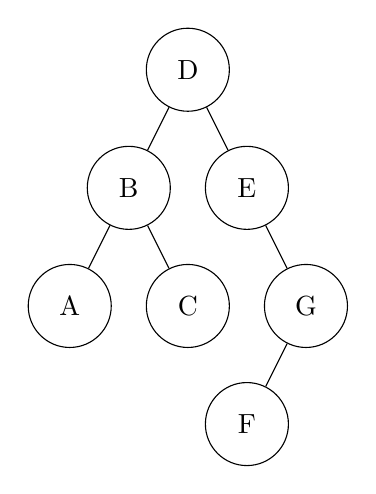
\begin{tikzpicture}[every node/.style={circle,minimum width = 30pt, minimum height =30pt, draw}]
        \node{D}
            child{node{B}
                child{node{A}}
                child{node{C}}}
            child{node{E}
                child[missing]{}
                child{node{G}
                    child{node{F}
                    child[missing]{}}
                    child[missing]{}
                }
            };
    \end{tikzpicture}
    \end{columns}
\end{frame}
\begin{frame}{1731 -- Orders (poj.org)}
    \begin{itemize}
        \item 给出字母序列,将这个序列中字母组成的所有可能排列/置换按字典序输出
    \end{itemize}
    \vfill
    \begin{exampleblock}{Sample}
        \begin{itemize}
            \item Sample Input: bbjd
            \item Sample Output: bbdj bbjd bdbj bdjb bjbd bjdb dbbj dbjb djbb jbbd jbdb jdbb
        \end{itemize}
    \end{exampleblock}
    \vfill
    \begin{itemize}
        \item 实现:
        \begin{enumerate}
            \item 递归(手写)
            \item C++ STL中的next\_permutation\footnote{\url{https://cplusplus.com/reference/algorithm/next_permutation/}}函数
        \end{enumerate}
    \end{itemize}
\end{frame}
\begin{frame}{2.3 分治法}
    \begin{block}{分治法}
        将原问题分解成规模较小但是与原问题类似的子问题,通过递归来求解这些子问题,再将子问题的解合并来求出原问题的解的方法
    \end{block}
    \vfill
    \begin{itemize}
        \item 分治在递归的过程中有三步:
        \begin{enumerate}
            \item 分解:将原问题分解成规模较小但是与问题类似的子问题
            \item 求解:递归求解子问题,子问题规模足够小时直接求解
            \item 合并:将子问题的解合并,求出原问题的解
        \end{enumerate}
    \end{itemize}
\end{frame}
\begin{frame}{MapReduce}
    \includegraphics[width=\textwidth]{fig/2-3.png}
\end{frame}
\begin{frame}{2388 -- Who's in the Middle (poj.org)}
    \begin{itemize}
        \item 求n个数的中位数,n为奇数
    \end{itemize}
    \vfill
    \begin{itemize}
        \item 分析
        \begin{enumerate}
            \item 如果n个数是有序的,那么第$\frac{n+1}{2}$个数就是所求的中位数
            \item 在C语言提供了排序函数qsort\footnote{\url{https://cplusplus.com/reference/cstdlib/qsort/}},C++语言提供了sort\footnote{\url{https://cplusplus.com/reference/algorithm/sort/}}, 它们的实现都是基于快速排序
            \item \textcolor{blue}{快速排序}(Quicksort),又称\textcolor{blue}{划分交换排序}(partition-exchange sort),简称\textcolor{blue}{快排}
        \end{enumerate}
    \end{itemize}
\end{frame}
\begin{frame}{快速排序}
    \begin{columns}
        \column{0.3\textwidth}
        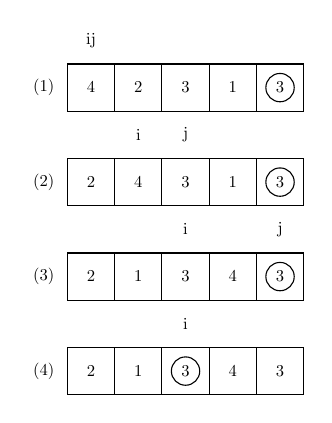
\begin{tikzpicture}[global scale=.6]
            \draw (-1,0) node{(4)};
            \draw (0,0) node[RA2]{2};
            \draw (1,0) node[RA2]{1};
            \draw (2,0) circle(.3) node[RA2]{3};
            \draw (3,0) node[RA2]{4};
            \draw (4,0) node[RA2]{3};
            \draw (2,1) node{i};
            \draw (-1,2) node{(3)};
            \draw (0,2) node[RA2]{2};
            \draw (1,2) node[RA2]{1};
            \draw (2,2) node[RA2]{3};
            \draw (3,2) node[RA2]{4};
            \draw (4,2) circle(.3) node[RA2]{3};
            \draw (2,3) node{i};
            \draw (4,3) node{j};
            \draw (-1,4) node{(2)};
            \draw (0,4) node[RA2]{2};
            \draw (1,4) node[RA2]{4};
            \draw (2,4) node[RA2]{3};
            \draw (3,4) node[RA2]{1};
            \draw (4,4) circle(.3) node[RA2]{3};
            \draw (1,5) node{i};
            \draw (2,5) node{j};
            \draw (-1,6) node{(1)};
            \draw (0,6) node[RA2]{4};
            \draw (1,6) node[RA2]{2};
            \draw (2,6) node[RA2]{3};
            \draw (3,6) node[RA2]{1};
            \draw (4,6) circle(.3) node[RA2]{3};
            \draw (0,7) node{ij};
        \end{tikzpicture}
        \column{0.7\textwidth}
        \begin{enumerate}[(1)]
            \item 选取数组a最右边元素作为基准值x,两个指针i和j最初都在序列最左边
            \pause
            \item 用a[j]和x的值进行比较,如果a[j]小于x,则交换a[i]和a[j],同时将i和j向右移动;如果a[j]大于等于x,则j右移,i不动
            \pause
            \item 当j移动到最右边时,i的左侧元素都小于x,右侧都大于等于x
            \pause
            \item 最后将x和a[i]值交换。序列就被i分成了左右两部分
            \pause
        \end{enumerate}
        交换过程结束后,两个3改变了之前的顺序,这种情况称为排序的不稳定性,所以这种快速排序算法是\textcolor{red}{不稳定}的排序算法
    \end{columns}
\end{frame}
\begin{frame}{2299 -- Ultra-QuickSort (poj.org)}
    \begin{itemize}
        \item 通过交换相邻元素进行排序,对于一个给定的无序序列a[1…n],计算最终完成升序排列需要交换的次数
    \end{itemize}
    \vfill
    分析
    \begin{enumerate}
        \item \textcolor{blue}{冒泡排序},所求的交换次数也就是计算无序序列的\textcolor{blue}{逆序对}数目,冒泡排序的时间复杂度是$O(n^2)$
        \item 求逆序对数目效率更高的方法是利用\textcolor{blue}{归并排序},可以做到$O(nlogn)$的时间复杂度
        \item 归并的具体方法是将排好序的两个数组的元素依次比较,将其中较小的依次放入一个辅助数组b中,因为两个数组已经排序,比较的过程直接从左边到最右边即可。最后用b替换原来的a,进行上一层的合并操作
    \end{enumerate}
\end{frame}
\begin{frame}{二分查找}
    \begin{tikzpicture}[
        hv/.style={to path={-| (\tikztotarget)},->,thick},
        h/.style={dashed,thick}]
        \draw (1,1) node[RA2]{1};
        \node[RA2](1) at(2,1) {3};
        \node[RA2](2) at(3,1) {4};
        \node[RA2](3) at(4,1) {6};
        \node[RA2](4) at(5,1) {7};
        \draw (6,1) node[RA2]{8};
        \draw (7,1) node[RA2]{10};
        \draw (8,1) node[RA2]{13};
        \draw (9,1) node[RA2]{14};
        \node (5) at (4,2.5) {4<6} edge[hv] (2) edge[h] (3);
        \node (6) at (2,3.5) {4>3} edge[hv] (5) edge[h] (1);
        \node (7) at (5,4.5) {4<7} edge[hv] (6) edge[h] (4);
        \node at (5,5.5) {} edge[hv] (7);
    \end{tikzpicture}
\end{frame}
\begin{frame}{1905 -- Expanding Rods (poj.org)}
    \begin{itemize}
        \item 细棒长度$L$,两端固定,加热后膨胀为一段圆弧,长度变为
        $$L'=(1+n\cdot C)\cdot L$$
        $n$为变化的温度,$C$为膨胀系数,求细棒中心移动的距离
    \end{itemize}
    \vfill
    \begin{center}
        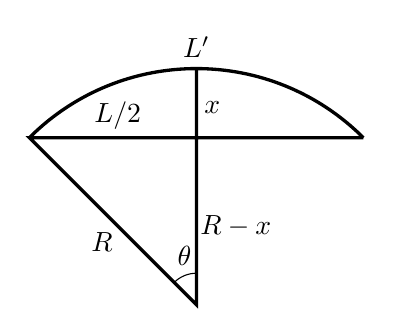
\begin{tikzpicture}
        \draw[very thick] (2.12,2.12) arc (45:135:3) node[midway,above]{$L'$};
        \draw[very thick] (0,3)--(0,0)--(-2.12,2.12)--(2.12,2.12);
        \draw (0,.4) arc (90:135:.4) node[midway,above]{$\theta$};
        \node at (.5,1){$R-x$};
        \node at (.2,2.5){$x$};
        \node at (-1,2.4){$L/2$};
        \node at (-1.2,.8){$R$};
    \end{tikzpicture}
    \end{center}
\end{frame}
\begin{frame}{1905 -- Expanding Rods (poj.org)}
    \begin{center}
       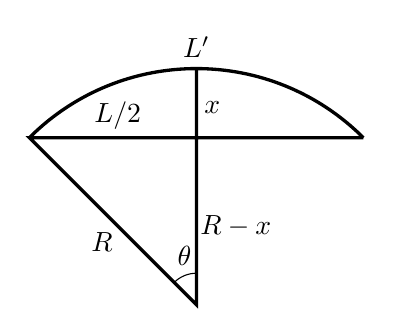
\begin{tikzpicture}
        \draw[very thick] (2.12,2.12) arc (45:135:3) node[midway,above]{$L'$};
        \draw[very thick] (0,3)--(0,0)--(-2.12,2.12)--(2.12,2.12);
        \draw (0,.4) arc (90:135:.4) node[midway,above]{$\theta$};
        \node at (.5,1){$R-x$};
        \node at (.2,2.5){$x$};
        \node at (-1,2.4){$L/2$};
        \node at (-1.2,.8){$R$};
    \end{tikzpicture} 
    \end{center}
    $$R^2=(R-x)^2+(L/2)^2\Rightarrow R=\frac{x^2+(L/2)^2}{2x}$$
	$$sin⁡θ=\frac{L/2}{R}\Rightarrow θ=sin^{-1}(\frac{L/2}{R})$$
	\center{代入 $L'=2Rθ$ 可得$x$和$L'$的关系}
\end{frame}
\begin{frame}{三分查找}
    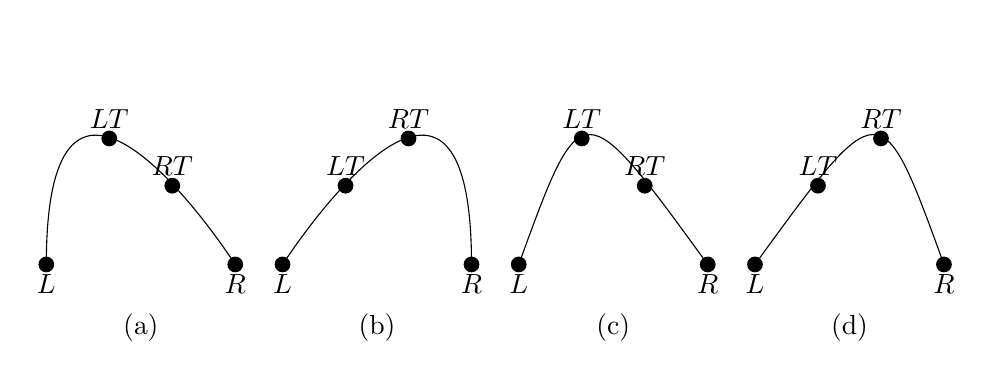
\begin{tikzpicture}
        \foreach \x in {0,1,2,3}{  
            \fill   ($(0,0)!\x*.25!(12,0)$) circle (.1) node[below]{$L$}
                    ($(2.4,0)!\x*.25!(14.4,0)$) circle (.1) node[below]{$R$}
                    ($(0.8,0)!\x*.25!(12.8,0)!abs(cos(\x*90))*.3+.5!(0.8+3*\x,2)$) circle (.1) node[above]{$LT$}
                    ($(1.6,0)!\x*.25!(13.6,0)!abs(sin(\x*90))*.3+.5!(1.6+3*\x,2)$) circle (.1) node[above]{$RT$};}
        \draw (0,0) ..controls (0,3) and (1.6,1.2)..(2.4,0);
        \draw (5.4,0) ..controls (5.4,3) and (3.8,1.2)..(3,0);
        \draw (6,0) ..controls (6.8,2.2)..(8.4,0);
        \draw (11.4,0) ..controls (10.6,2.2)..(9,0);
        \node at(1.2,-.8) {(a)};
        \node at(4.2,-.8) {(b)};
        \node at(7.2,-.8) {(c)};
        \node at(10.2,-.8) {(d)};
    \end{tikzpicture}
    \begin{itemize}
        \item 由(a)(c)可以看出,f(LT)大于f(RT)时,可以将右侧区间删掉
        \item 由(b)(d)可以看出,f(LT)小于f(RT)时,可以将左侧区间删掉
    \end{itemize}
\end{frame}
\begin{frame}{2420 -- A Star not a Tree? (poj.org)}
    \begin{itemize}
        \item 给出平面上n个点的坐标,找到一点,到这些点的距离和最小
    \end{itemize}
    \vfill
    \begin{itemize}
        \item 分析
        \begin{enumerate}
            \item 所求的就是几何学中的\textcolor{blue}{费马点},显然几何方法不适用于计算机,在空间范围内搜索该点,可以采用分治策略进行,不断缩小求解空间,直到找到符合精度要求的解
            \item 本题的坐标空间x和y都在0到10000之间,随着x和y的增加,解并不是单调变化,无法用二分搜索来实现。问题区间不满足单调性,但是符合\textcolor{blue}{凸函数},的性质,求区间最值可以采用三分的方法
        \end{enumerate}
    \end{itemize}
\end{frame}
\end{document}